% !TEX TS-program = pdflatex
% !TEX encoding = UTF-8 Unicode

% This is a simple template for a LaTeX document using the "article" class.
% See "book", "report", "letter" for other types of document.

\documentclass[11pt]{article} % use larger type; default would be 10pt
\usepackage[utf8]{inputenc} % set input encoding (not needed with XeLaTeX)

%%% Examples of Article customizations
% These packages are optional, depending whether you want the features they provide.
% See the LaTeX Companion or other references for full information.

%%% PAGE DIMENSIONS
\usepackage{geometry} % to change the page dimensions
\geometry{a4paper} % or letterpaper (US) or a5paper or....
% \geometry{margin=2in} % for example, change the margins to 2 inches all round
% \geometry{landscape} % set up the page for landscape
%   read geometry.pdf for detailed page layout information

\usepackage{graphicx} % support the \includegraphics command and options

% \usepackage[parfill]{parskip} % Activate to begin paragraphs with an empty line rather than an indent

%%% PACKAGES
\usepackage{booktabs} % for much better looking tables
\usepackage{array} % for better arrays (eg matrices) in maths
\usepackage{paralist} % very flexible & customisable lists (eg. enumerate/itemize, etc.)
\usepackage{verbatim} % adds environment for commenting out blocks of text & for better verbatim
\usepackage{subfig} % make it possible to include more than one captioned figure/table in a single float
% These packages are all incorporated in the memoir class to one degree or another...

%%% HEADERS & FOOTERS
\usepackage{fancyhdr} % This should be set AFTER setting up the page geometry
\pagestyle{fancy} % options: empty , plain , fancy
\renewcommand{\headrulewidth}{0pt} % customise the layout...
\lhead{}\chead{}\rhead{}
\lfoot{}\cfoot{\thepage}\rfoot{}

%%% SECTION TITLE APPEARANCE
\usepackage{sectsty}
\allsectionsfont{\sffamily\mdseries\upshape} % (See the fntguide.pdf for font help)
% (This matches ConTeXt defaults)

%%% ToC (table of contents) APPEARANCE
\usepackage[nottoc,notlof,notlot]{tocbibind} % Put the bibliography in the ToC
\usepackage[titles,subfigure]{tocloft} % Alter the style of the Table of Contents
\renewcommand{\cftsecfont}{\rmfamily\mdseries\upshape}
\renewcommand{\cftsecpagefont}{\rmfamily\mdseries\upshape} % No bold!

%%% END Article customizations
\usepackage{xcolor}
\usepackage{tcolorbox}
\usepackage{lipsum}  % 示例文本
\usepackage{mdframed}
\usepackage{pdfpages}


% R code support
\usepackage{listings}
% \lstset{language=R,  % 设置语言为R
%         basicstyle=\ttfamily, % 设置字体样式
%         numbers=left,  % 行号显示在左侧
%         numberstyle=\small\color{blue},  % 行号样式
%         frame=single,  % 设置代码块的边框
%         backgroundcolor=\color{lightgray},  % 设置代码块的背景颜色
%         }

\usepackage{graphicx}
\usepackage{float}
\usepackage{amsmath}





% 设置R语言代码高亮
\lstdefinestyle{rstyle}{
  language=R,
  basicstyle=\ttfamily,
  numbers=left,
  numberstyle=\tiny\color{gray},
  commentstyle=\color{green!40!black},
  keywordstyle=\color{blue},
  stringstyle=\color{purple},
  morekeywords={read.csv},
  frame=single,
  breaklines=true
}
% 

\title{Introduction to Statistics for DS \\ 
Groupwork-Based Assignment 1}
% 
\author{Durham Student ID: \textbf{001102553}, IT account: \textbf{bjsn39}}
\begin{document}
\maketitle

% % Question 1 with 4 multi-choice
\section{Question 1}
% \paragraph{\textcolor{red}{I've highlight the keywords and calculation steps in the questions part.}}
\paragraph{1. B}
\paragraph{\textbf{Analytics:}  The answer options "0," "1," "2," and "3 or more" represent an ordered range, but the gaps between them are not necessarily equal. In this case, the data is ordered, but cannot perform exact mathematical operations, and is therefore classified as ordinal data.}
\paragraph{2. A}
\paragraph{\textbf{Analytics:} Not interested in the proportion each continent of origin make up.}
% 
\paragraph{3. B}
\paragraph{\textbf{Analytics:} Let Event A = British population said they preferred dogs to cats, \\ Event B = British population
    listed jazz as one of their favourite musical genres. \\
    A and B are mutual independent $\Rightarrow$ $P(AB)=P(A)P(B)=46\%*12\%=5.52\%$ }
\paragraph{4. A}
\paragraph{{\textbf{Analytics:} $P(A \cup B)=P(A)+P(B)-P(AB)=\frac{4}{7}+\frac{5}{7}-\frac{6}{7}=\frac{3}{7}$}}
\paragraph{5. D}
\paragraph{{\textbf{Analytics:}
            \begin{equation*}
                F(u) =
                \begin{cases}
                    \frac{u^2}{4} \bigg |_{low}^{high} & \text{if } 0 \leq u \leq 2 \\
                    0                                  & \text{otherwise }
                \end{cases}
            \end{equation*}
            \begin{equation*}
                P(u>0.30)=\frac{u^2}{4} \bigg |_{0.30}^{2}=1-\frac{0.09}{4}=0.9775
            \end{equation*}
        }}
% \section{Question 2}
\subsection{Find the modal tooth length across the entire data set.}
\begin{lstlisting}
# clear the console area
cat("\014")

# clear the environment var area
rm(list = ls())

# Load the Tooth Growth data set
data(ToothGrowth

# Find the modal tooth length
modal_tooth_length1 = as.numeric(names(sort(
    table(ToothGrowth$len), decreasing = TRUE)[1]))
\end{lstlisting}
% 
\subsection{Mean tooth length for guinea pigs who were given their vitamins via orange juice}
% 
\begin{lstlisting}
# Calculate the mean tooth length for guinea pigs 
# given vitamins via orange juice
mean_tooth_length_orange = mean(
    ToothGrowth$len[ToothGrowth$supp == "OJ"])
mean_tooth_length_orange    
\end{lstlisting}
% 
\subsection{Create a side-by-side box-and-whisker plot:}
% 
\begin{lstlisting}
# Create a side-by-side box-and-whisker plot
# for tooth length by supplement type
boxplot(len ~ supp, data = ToothGrowth, 
        col = c("lightblue", "lightgreen"),
        xlab = "Supplement Type", ylab = "Tooth Length",
        main = "Tooth Length by Supplement Type")
legend("topright", 
        legend = c("Ascorbic Acid", "Orange Juice"), 
        fill = c("lightblue", "lightgreen"))
\end{lstlisting}
% 
% 
\begin{figure}[H]
    \centering
    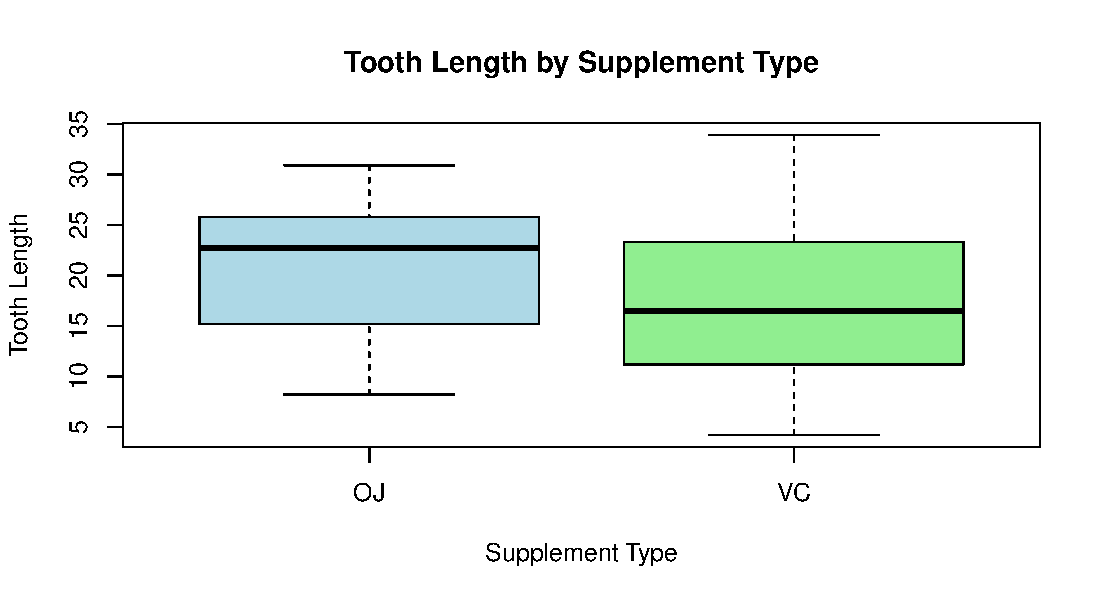
\includegraphics[width=0.8\textwidth]{img/ToothLength.pdf}
    % \caption{}
    % \label{fig:your-label}
\end{figure}
% 
% 
\subsection{Comment on which vitamin delivery approach is more effective:}
\paragraph{To determine which vitamin delivery approach is more effective in promoting tooth growth, you should analyze the box-and-whisker plot created in the previous step. Look at the distribution of tooth lengths for guinea pigs given vitamins via ascorbic acid and orange juice.
If the median tooth length for one group is higher than the other, it suggests that the corresponding supplement may be more effective.
Additionally, look for differences in the spread (interquartile range) and the presence of outliers. A supplement with a larger median, smaller spread, and fewer outliers may be considered more effective.}
% \section{Question 3}
\subsection{Expected number of party poppers}
$$ E(X)=Probability\ of\ failure * Total\ number\ of\ party\ poppers $$
$$ E(X)=0.6\% *200=1.2 $$
% 
\subsection{Distribution of fail poppers}
\subsubsection{Poisson distribution}
\paragraph{To represent the number of party poppers that fail to go off in a box as a random variable, X, we can use the Poisson distribution. In this case, the Poisson distribution is appropriate because it models the number of events (party poppers failing to go off) that occur in a fixed interval (a box of party poppers) when the events are rare and random.}
% 
\paragraph{The parameter, $\lambda$ (lambda), is the average number of events in the fixed interval. Here, $\lambda$ is equal to the expected number of party poppers that will fail to go off, which was calculated in Part 1.}
% 
% 
\subsubsection{The assumptions that need to hold for justifying the use of the Poisson distribution}
\begin{itemize}
    \item Events (party poppers failing to go off) occur randomly.
    \item Events are rare, meaning the probability of more than one event occurring in a very short time period is negligible.
    \item Events are independent of each other.
\end{itemize}
% 
% 
% 
\subsection{Distribution of mistake box}
\subsubsection{Distribution for Y}
\paragraph{For the random variable Y, representing the number of party poppers that fail to go off in a box of 2 (due to the administrative error), you can still use the Poisson distribution with the same $\lambda$ value as calculated in Question 3.1, which is based on the company's claim.}

\subsubsection{$E(Y)$ and $Var(Y)$}
\paragraph{According to Poisson Distribution, PMF is:}
$$ P(Y=k)=\frac{e^{- \lambda} \lambda^k}{k!} $$
$$ E(Y)= \mu = \lambda $$
$$ Var(Y) = \sigma^2 = \lambda $$
% \section{Question 4}
\subsection{Calculate $P(X=4)$}
\paragraph{Poisson probability formula is: $ P(X=k)=\frac{e^{- \lambda} \lambda^k}{k!} $}
\paragraph{In this case, $k=4$ and $\lambda=0.4$:}
$$ P(X=4)=\frac{e^{-0.4}*0.4^4}{4!}=0.000715008 $$
\subsection{Calculate $P(X<3)$}
$$ P(X<3)=P(X=0)+P(X=1)+P(X=2) =0.9920737 $$
\subsection{Calculate $P(Y=4 | Y \ge 3)$}
\paragraph{The conditional probability of an event A given event B is defined as:}
$$ P(A|B)=\frac{P(AB)}{B}$$
\paragraph{The $P(Y=4 | Y \ge 3)$ equals to $\frac{P(Y=4 \cap Y \ge 3)}{P(Y \ge 3)}$}
% 
\begin{equation*}
    \left.
    \begin{array}{ll}
        P(Y=4 \cap Y \ge 3) = P(Y=4) \\
        P(Y \ge 3)=1-P(Y < 3)
    \end{array}
    \right\}
    \Rightarrow
    P(Y=4 | Y \ge 3)=\frac{0.000715008}{1-0.9920737}=0.090207
\end{equation*}
\textbf{An easier way to Calculate via R}
% 
\begin{lstlisting}[style=rstyle]
# set lambda
lambda = 0.4

# calculatP(X = 4)
probability <- dpois(4, lambda)
cat("P(X = 4) =", probability, "\n")

# calculateP(X < 3)
probability <- ppois(2, lambda)
cat("P(X <3) =", probability, "\n")
\end{lstlisting}
\paragraph{Throughout my 4-week journey in the ISDS module, I have embarked on a compelling exploration of groupwork. This assignment serves as an opportunity to reflect on the profound impact of groupwork, recounting experiences that have not only broadened my understanding but also reshaped my perspective on collaborative endeavors with classmates from different countries.}
% 
% 
\section{A Contribution That Benefited Our Group}
% 
\paragraph{Before the start of the second week, I checked the group assignment results on the Ultra platform and was excited to find out my group members. I was the first to reach out to my group members by sending a self-introduction message in the Messages section. This message included my basic personal information and a link to my personal homepage. I was pleased to take the initiative, and my group members were very welcoming. In the days leading up to the start of the class, everyone introduced themselves in the chat box. One of my group members even praised my well-crafted GitHub page. Subsequently, we established a WhatsApp group, which laid a strong foundation for future communication.}
% 
\paragraph{During the second week's ice-breaking activity, our prior interactions proved invaluable. We all participated actively in the activity, and there was no hint of awkwardness, thanks to the positive rapport we had established earlier.}
% 
% 
% 
% 
\section{My Belbin Role in Group Work}
% 
\paragraph{Regarding my role within the team, I believe I embody both the \textbf{Completer Finisher} (CF) and \textbf{Specialist} (SP) roles.}
% 
\paragraph{Firstly, as a Completer Finisher, I consistently deliver high-quality results in any form of assignment. Perhaps owing to my inclination towards perfectionism, I prefer using LaTeX for typesetting (this assignment, for instance, was created using LaTeX), and I utilize specialized software like Tikz and draw.io to produce intricate graphics. As with my first personal assignment, I'm used to using LaTeX to edit formulas instead of taking pictures of my ugly handwritten formulas. Additionally, I play an effective role in motivating the team. For instance, in the process of completing this group-based individual assignment, I proactively scheduled a Zoom meeting with my team members to facilitate discussion and ensure a better outcome.}
% 
\paragraph{Secondly, I also consider myself eligible to be a Specialist. My life's motto is: "If something needs to be calculated more than five times, I will write a program for it rather than performing manual calculations." I intend to uphold the same approach in our group assignments.}
% 
% 
% 
% 
% 
% 
% 
\section{Another Group Member Act in Belbin's role}
% 
\paragraph{It's worth mentioning that there's a notable team member in our group, whom I will refer to as "Z," as it's the initial letter of her name. I believe she embodies the qualities of an excellent Team Worker. In the third week, when a team member from our group decided to switch to another major, she was the first to communicate and confirm this news with the student changing majors. This demonstrated her genuine concern for the well-being of our team members. }
% 
\paragraph{Moreover, whenever a message is posted in our WhatsApp group, she consistently responds with enthusiasm, which is a great way to motivate the team. I consider Z to be a reliable teammate, and I am eager to collaborate with her in the future.}
% 
% 
% 
% 
\section{Lessons from Group Work}
% 
\paragraph{As the deadline for assignment submissions approaches, I often find myself experiencing a sense of anxiety. I tend to meticulously refine our content, even our formatting, in a quest for perfection. Consequently, I have been discussing with our group members the possibility of establishing a group deadline in the future. This would allow ample time for optimization and mitigate potential issues stemming from system errors that could lead to assignment submission failures. The goal is to ensure that when it comes time to submit our work, we do so with confidence.}
% 
% 
% 
% 
% 
% 
% 
% 
% 
% 
% 
% 
% 
% 
\newpage
\begin{mdframed}[
        backgroundcolor=white,  % 背景颜色
        linecolor=black,        % 边框颜色
        leftmargin=5pt,         % 左边距
        rightmargin=5pt,        % 右边距
        linewidth=2pt           % 边框的宽度
    ]
    \textbf{Reflecting on My Group Experience: Insights and Observations}
    \begin{itemize}
        \item I consider myself fortunate to have observed that, thus far, our group members have exhibited remarkable enthusiasm and the willingness to voice their opinions in group work. A recent Zoom discussion we had regarding this assignment is a testament to this positivity. Only one member was absent due to health reasons, but they promptly explained their situation in our WhatsApp group and inquired about the discussion content. I believe we have fostered a conducive group atmosphere. If we can sustain this atmosphere, I am confident we will achieve commendable results in our upcoming group tasks.
        \item As a newcomer to R programming, despite having prior experience with languages like Python and JavaScript, I still grapple with certain programming paradigms. Thankfully, our group member "C" has been exceptionally eager to help me understand and has been quick to address my queries during seminars. I am grateful for their support.
    \end{itemize}
    % 
\end{mdframed}
% 
% 
% 
% 
% 
% 
% 
% 
% 
% 
% 
% 
% 
% 
% 
% 
\begin{mdframed}[
    backgroundcolor=white,  % 背景颜色
    linecolor=black,        % 边框颜色
    leftmargin=5pt,         % 左边距
    rightmargin=5pt,        % 右边距
    linewidth=2pt           % 边框的宽度
]
\textbf{Constructive Criticism for Improvement: }
Initially, we found it challenging to complete the worksheets during the seminars, especially for individuals like us who are newcomers to R programming. Balancing statistical theory knowledge and R language coding proved to be demanding. However, our team wisely heeded the advice of another high-performing group member, who happened to be my friend. Although we were not in the same group, he generously shared his experiences. His recommendation was to first complete the online course on Ultra and try to address the worksheet questions before the classes. Following this advice, we found ourselves much better prepared and at ease by Week 4.
% 
\end{mdframed}
% 
% 
% 
% 
% 
% 
% 
% 
% 
% 
% 
\end{document}
